\subsection{Composer un plat}

\noindent \textbf{Nom:} Composer un plat \\
\textbf{ID:} UC401\\
\textbf{Description :} Le diététicien souhaite pouvoir composé un plat (petit-déjeuner, déjeuner, souper) en renseignant sa composition.\\
\textbf{Auteurs :} Nicolas SYMPHORIEN\\
\textbf{Date :} 16/06/2017 \\
\textbf{Acteurs :} Le diététicien \\
\textbf{Pré-condition :} \\
Le diététicien doit être connecter (Voir le cas d'utilisation secondaire ``S'authentifier''). \\
La liste des plats doit être accessible.

\noindent \textbf{Scénario principal : } Figure \ref{ComposerPlatSeq}

\begin{enumerate}
	\item \label{UC401_step1}Le système affiche la liste des plats déjà crée.
	\item \label{UC401_step2}Le diététicien choisi de créer un nouveau plat.
	\item Le système affiche une page permettant d'entrer les ingrédients composant le plat ainsi que leurs quantités
	\item Le diététicien choisi les ingrédients qu'il veut mettre dans son plat
	\item Le système enregistre le plat crée et affiche un message de confirmation de création
\end{enumerate}

 \noindent \textbf{Scénario alternatif :}

Les deux scénario alternatifs débute après l'étape \ref{UC401_step1} du scénario nominal.
\begin{enumerate}
	\item Le diététicien choisi de modifier un plat déjà existant.
	\begin{enumerate}
		\item Le système affiche les ingrédients du plat à modifier
		\item Le diététicien modifie la composition du plat et confirme les modifications
		\item Le système enregistre le plat modifié et affiche un message de confirmation de modification
	\end{enumerate}
	\item Le diététicien choisi de supprimer un plat déjà existant.
	\begin{enumerate}
		\item Le système affiche un message d'avertissement avant la suppression
		\item L'utilisateur confirme la suppression du plat
		\item Le système supprime le plat modifié et affiche un message de confirmation de suppression
	\end{enumerate}
\end{enumerate}
Dans les deux cas, le cas d'utilisation reprend à l'étape \ref{UC401_step2} du scénario nominal.

\noindent \textbf{Post-Conditions:} Le plat est crée, modifié ou supprimé.

\begin{figure}
\centering
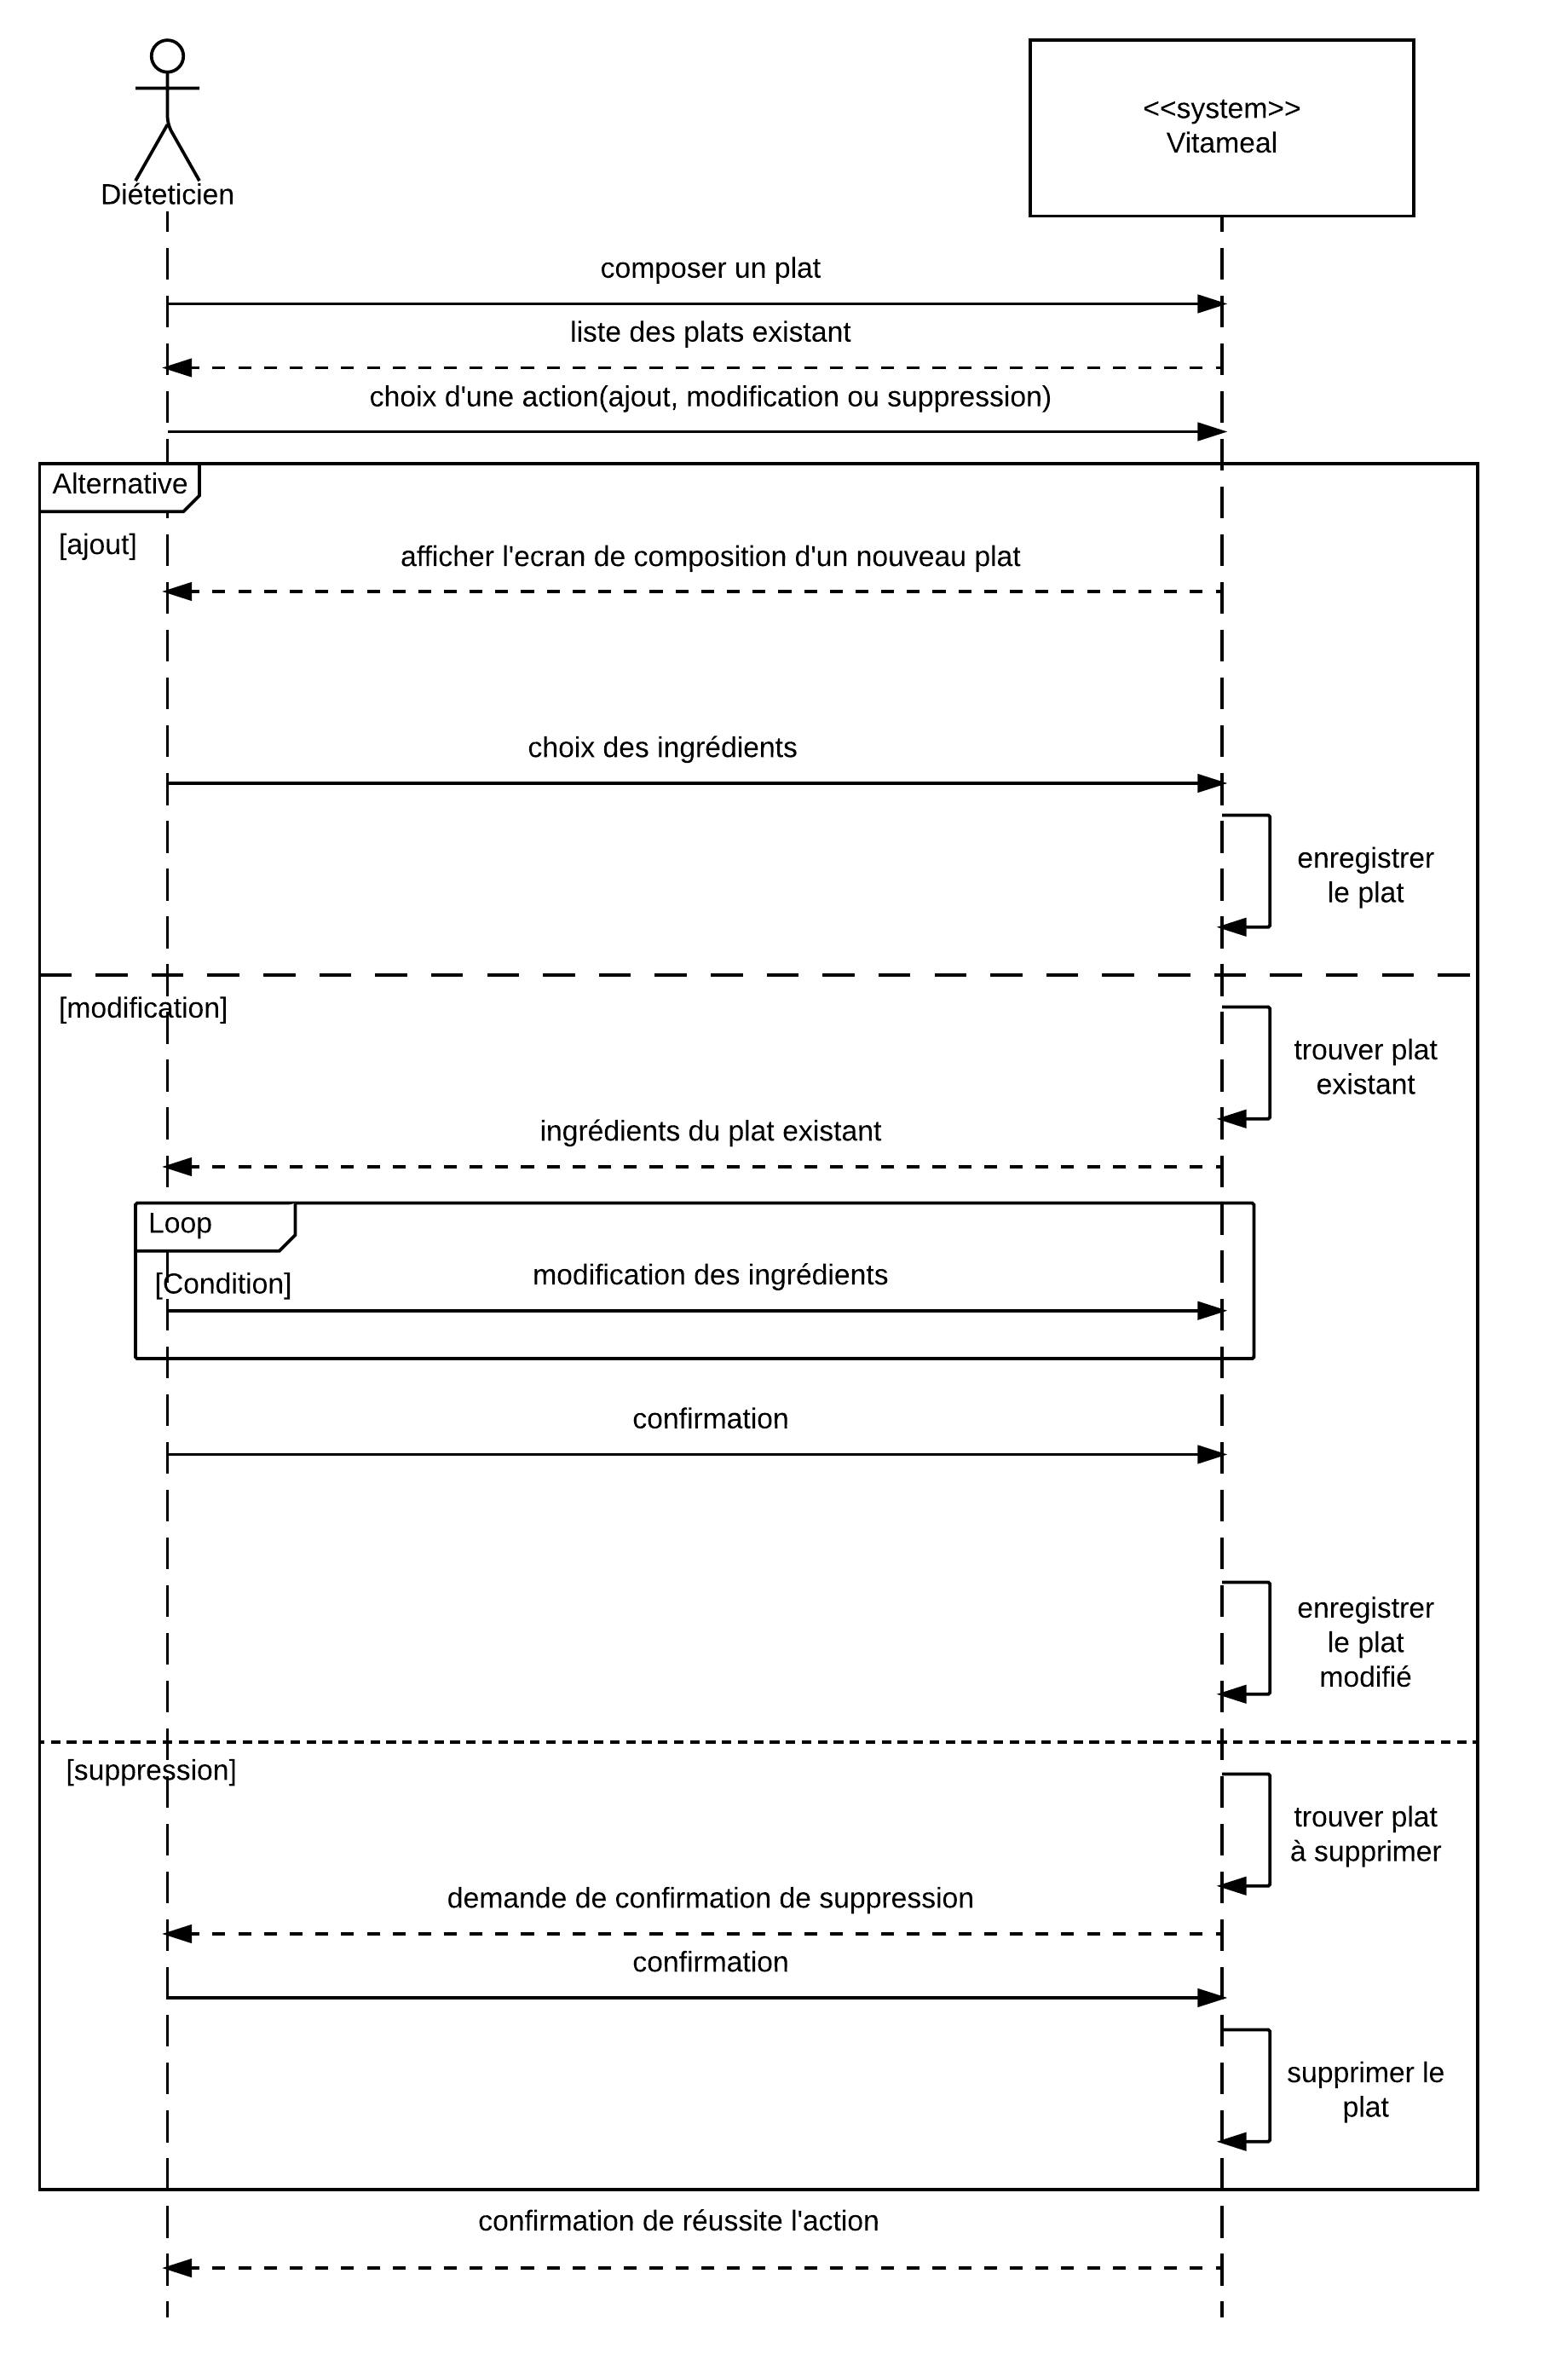
\includegraphics[scale=0.3]{../../CasDUtilisations/CompositionPlat/sequence_UC_ComposerPlat.png}
\caption{Diagramme de séquence du cas d'utilisation composer un plat}
\label{ComposerPlatSeq}
\end{figure}
